\chapter{Background}
\label{sec:background}
In this chapter, the main focus is on the basics concepts used in the thesis. We will start with the basic process of machine learning, what are the types of attacks exist for it. Then some concepts about TEEs and differential privacy are explained which we will use to develop our system SPML.
\section{Machine learning}
Machine learning \cite{65} aims to build a system that learns with experience. It is a mix of statistics and computer science. Machine learning is widely used in every field of technology, science, and commerce such as education, health care, finance policing, marketing, etc. The machine learning comes under the study of artificial intelligence. Many Artificial intelligence (AI) based systems such as speech recognition, computer vision, robot control, natural language processing are using machine learning for their software development. Machine learning consists of data or database as an input, a training model, and predictions/classification as output. It consists of two phases training phase and the inference phase. The training phase trains the model with the help of input data and the inference phase is the one in which this trained model is used to predict/classify the real-world problem. These phases are discussed in brief as follows.

\subsection{Training Phase}
In this phase, the model is trained to predict output or classify something such as an image. It consists of reading the input, prepossessing the input (making it suitable to feed into the model), defining a model, choosing a loss function, and an optimizer. The model has some parameters which help to deduce output based on the input. For example, to predict the average salary of an individual, the input can be education qualification, years of working experience, occupation, etc, and output will be salary. 

\begin{figure}
    \centering
    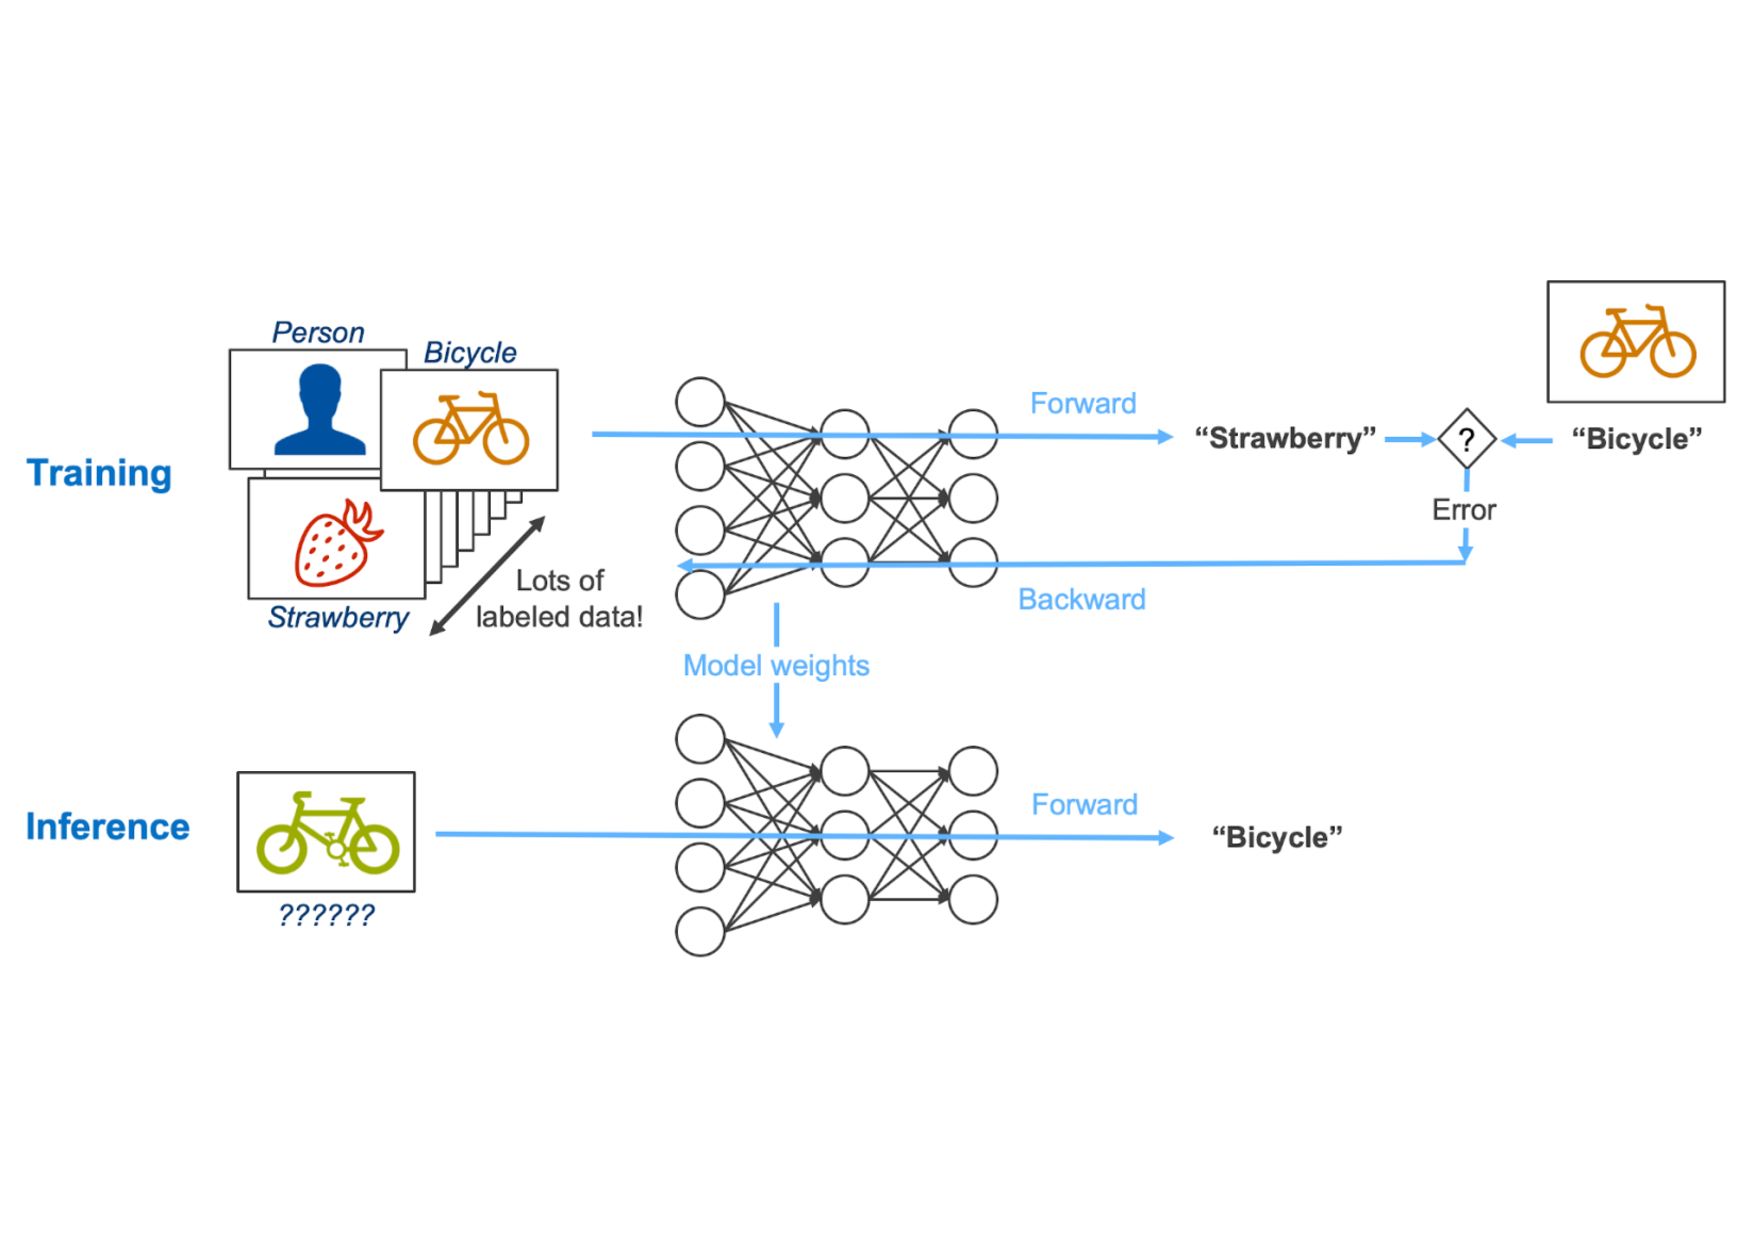
\includegraphics[width=10cm, height=10cm]{images/Background/config.pdf}
    \vspace{-6em}
    \caption{Training vs Inference Phase \cite{82}}
    \label{fig:backgroundTI}
\end{figure}

In general, the training phase tries to find the nth (column) point using (n-1) points (columns). The input data set is made up of some n points (columns). The main goal of training is to find the optimal settings to achieve the maximum accuracy so that the nth point can be predicted/classified correctly using n-1 points. The goal of the loss function is to find how well the current model is performing on predicting/classifying the target (training) data. For example, if there is too much deviation from the expected value, then the loss function will be very high. On the other hand, the optimizer function helps to minimize this loss. Hence, the training phase includes the main computation where the loss function calculates the loss or deviation from the expected values, and the optimizer function tells how to minimize the loss by adjusting various model's parameters. The adjustment of the model's parameters is a lengthy process and takes multiple iterations to find the optimal values. The accuracy of the model is calculated using these model's parameters and is an important parameter to decide when to stop the training.

For example, in Figure ~\ref{fig:backgroundTI} the neural network is trained to classify images into three categories which can be a strawberry, a bicycle, and a person. The training data has a lot of images and these images are labeled as strawberry, bicycle, and person. Each of the images will be passed through different layers of network and the network is trying to classify these images into a person, bicycle, or strawberry. It might be possible that during the training a bicycle image is classified as strawberry which is incorrect. To handle this, the error will be propagated back to the network, and model weights are corrected so that the next time model classifies the image into the correct category. This process continues where images are fed to the network and weights will be updated again and again to correct such errors. The training process is continued until the model is achieving the desired accuracy level. Once the model is trained with sufficient accuracy it can be used to inference, which forms the next phase of any machine learning system.
 

\subsection{Inference Phase}
This phase act on the trained model obtained from the training phase to predict/classify unseen data. The trained model is of small size and hence can be easily deployed in any device or computing platform such as cloud or smartphones, etc. It can be used to inference real-world data. With a well-trained model, one should get almost the same accuracy with real-world data as got during the training phase. Its a compress, simple, and optimized version of the training phase. For example, in Figure ~\ref{fig:backgroundTI}, when the image is fed into the trained model, the model classifies correctly it as a bicycle. The model uses model weights obtained from the training phase to make an inference.

In terms of performance, the inference phase is much faster than the training phase because, in the inference phase, we don't need to adjust any model's parameters which is the most time-consuming part in the whole machine learning process. A well-trained model will be able to do right predictions as much as possible for real-world data. Despite all the advantages that machine learning offers it also suffers from a few challenges such as the curse of dimensionality.

\subsection{Challenge of machine learning}
Machine learning cannot solve many important problems of AI such as speech or object recognition \cite{65}. Machine learning problems don't perform or fit well when the data has a lot of dimensions. This problem of high dimension is called a curse of dimensionality. If there are more dimensions there will be more variables and machine learning algorithms don't perform well in such scenarios. Machine learning algorithms have high computation costs and cannot learn complex functions in such high dimensional spaces. Hence machine learning cannot generalize all the problems in AI. To address such issues and apply machine learning in general, deep learning technique is widely used to solve the aforementioned problems.

\subsection{Deep learning}
Deep learning is a specific type of machine learning \cite{65}. It aims to solve the problem in representation learning such as speech or object recognition. It tries to present these representations into more simple representations so that complex concepts can be built out of simpler ones. To get an idea about this concept, let us understand the basic model in deep learning knows as multilayer perception (MLP). It maps input values to output values. It consists of a much simpler function and together they compose further complex functions. 

For example, if we take image classification then, the computer cannot understand the sensor input as an image. However, images can be represented as a collection of pixels. Deep learning breaks this complex problem into many nested mappings. All these nested mappings can be described by a different layer in the model. The first layer generally known as the input layer holds observable values. Thereafter, other features from the image are extracted by hidden layers after the input layer. With the help of pixels, input layers can detect edges of the images. Once edges are detected next hidden layer can detect for corners and contours and then the next hidden layer can detect specific objects. Once the object is detected, it is easy to identify if that object is a part of the image or not. Hence the complex problem is solved by dividing the problem into multiple stages or layers. This is how deep learning solves any kind of problem which can be speech, object recognition, or simple prediction problem.

Machine learning and deep learning are related to each other. Briefly, we can say machine learning is one approach to build AI systems and deep learning is a kind of machine learning that provides flexibility in representing real-world problems. However, machine learning/deep learning is not free from attacks, an adversary can try to steal the data from the training set or poison the data to sabotage the training process. We need to protect our data, model, and computation with all such attacks. To protect our machine learning or deep learning system against such attacks, first, we need to understand how various attacks can happen over these systems.

\subsection{Attacks on machine learning}
\label{sec:attackOnML}
In this subsection, our focus will be on privacy attacks on the machine learning system. In general, to attack a database and to gain private information inference attacks \cite{71} are commonly used. In this attack, data is analyzed to gain knowledge of an individual or subject. For example, the adversary can query the database to gain some group information and with some prior knowledge about the subject, it can infer information with the help of multiple summary statistics queries such as COUNT, SUM, or AVERAGE \cite{72}. Machine learning is purely based on the training model on some datasets/database, hence machine learning models can be attacked using inference attack easily. Some popular inference attacks known for machine learning are as follows.
\subsubsection{Model inversion attack}
In model inversion attack, as stated in \cite{17}, if an adversary has access to a trained model and some auxiliary information about an individual then it can make predictions about an individual's genetic markers. This particular attack is discussed via an example from the pharmacogenetics field in the paper, but it can be generalized for any scenario. It is assumed that only researchers have access to datasets and only the model learned from these datasets is made public. It is a black box type of attack, datasets are private and not accessible by an adversary. However, an adversary can exploit the correlation between unknown attributes, model output, and target information. This means an adversary has access to a trained model only and using this model it can easily deduce input attributes passed to the model.

It is a security and privacy risk to the applications based on such trained models. It is proved in the paper that, if an adversary knows the intended individual's background and dosage, then it can predict their genetic markers with good accuracy. This will compromise the privacy of an individual and we need to protect that. To prevent such attacks, the author used state-of-the-art differential privacy mechanisms to produce trained models and it was concluded that genomic privacy is protected for a small value of $\epsilon$. Hence, to some extent, such attacks can be prevented using differential privacy.

\subsubsection{Membership inference attack}
Membership inference attack, \cite{16} states that if access is given to a machine learning model, then is it possible to determine whether a record was used to train this model is present or absent in the training dataset. It is a black box type of attack where an adversary can only fire queries to get output for the given input. In this attack, machine learning is used against itself. 

Authors used a technique called shadow training which creates shadow models. To develop training datasets for these models, there are few methods discussed in the paper \cite{16} and can be referred for more details. These model's behavior is then imitated for the target model. The attack model is trained using these shadow models which converts this inference problem into a mere binary classification problem. Authors have suggested that to mitigate such types of attacks differentially private models can be used. The differentially private trained models are immune to membership inference attacks like in this case where only model output is known and no auxiliary information is known to the adversary.

\subsubsection{Model extraction attack}
Model extraction attack \cite{73} is also a black box attack. In this, an adversary tries to steal the model functionality without knowing any training data or model's parameter. An adversary sees the model as a black box hence can query it. It can learn predictions on some input features by querying the model. It is also assumed that the adversary doesn't know about training data distribution or model type (linear regression, decision tree or logistic regression, etc). This attack is successfully demonstrated for majority model types such as logistic regressions, SVMs, decision trees, and deep neural networks. If differential privacy prevents such type of attack or not is left for further discussion.

After going through all these inference attacks which try to learn either model parameters or if a particular record is in the training set or not, differential privacy proved to be a successful mechanism to avoid or prevent these types of attacks. Hence, we decided to use differential privacy in our thesis to address the privacy concern. To understand what exactly is differential privacy, how to apply differential privacy, why it can avoid such attacks, we studied differential privacy in detail as explained below.
\section{Differential privacy}
Differential privacy (DP) \cite{3} was proposed by Cynthia Dwork from Microsoft research. It aims to learn desired information about a group while learning nothing about an individual in that group. This means that if an adversary tries to query some information out of this group, most of the responses will be equal, irrespective of any individual is present or absent in the group. For example, if a database of patient records is maintained by some hospital to indicate if some patient has cancer or not, then this information should not be leaked. However, if the hospital wants to release some data like the total number of patients with what type of cancer for research purposes. Then differential privacy defines if some adversary can intrude information then it shouldn't be learned that some particular individual has cancer. The assumption here is that the hospital is a trusted source and the database cannot be hacked by an adversary and hospitals want to protect patient privacy. Formally differential privacy is defined as:
\begin{itemize}
    \item $\epsilon$-\text{differential privacy} for some mechanism M:
        \begin{equation}
            \forall S , Pr[M(x) \in S] \leq exp( \epsilon ) . Pr[M(x') \in S]
        \label{eq:epsDP}
        \end{equation}
    where x, x' are any two neighboring data-sets, S $\subseteq$ range(M) and, $\epsilon$ is a measure of how much privacy is being leaked or also known as privacy loss.
    \item ($\epsilon$,$\delta$)-\text{differential privacy} for some mechanism M:
    \begin{equation}
        \forall S , Pr[M(x) \in S] \leq exp( \epsilon ) . Pr[M(x') \in S] + \delta
    \label{eq:epsdeltaDP}
    \end{equation}
    where $\delta$ is a small probability of failing.
\end{itemize}

After formally giving introduction and definition of DP, lets us discuss a few important qualities or properties which make DP an ideal mechanism to achieve privacy. There are many properties discussed in privacy book \cite{80} but here we will discuss only three properties which are important from this thesis point of view, these are :
\begin{itemize}
    \item  \textit{Composability}: If two or more independent components of a mechanism are differentially private then their union (composition) will also be differentially private.
    \item  \textit{Group privacy}: If the dataset has inputs that are correlated to each other, then privacy guarantees will be degraded gracefully.
    \item  \textit{Robustness}: The privacy guarantees are not dependent upon any kind of auxiliary information that is known to the adversary.
\end{itemize}

These properties make differential privacy special and important in achieving privacy. The next question is how we can achieve DP in our algorithms, what are different techniques to achieve it. Before discussing the techniques to achieve DP, let us discuss the sensitivity of a function that is used by these DP techniques to make any algorithm differentially private. In simple words, the DP is trying to hide if a particular person is present in the dataset or not. The presence or absence of one person shouldn't change the output. This means DP is trying to measure how much one individual can affect the output. Mathematically, we can say if there are two neighboring data sets say D1, D2 and some function f over D1 and D2, then \textbf{sensitivity of function f} is defined as how much this function f can change if applied on the D1 and D2 \cite{2}, this means we are trying to hide this difference, so sensitivity can be defined as:
\begin{equation}
\Delta f = \max(D1,D2) \mid f(D1)-f(D2) \mid
\label{eq:epsSentivity}
\end{equation}
The equation ~\ref{eq:epsSentivity} tells till what extend noise is added so that privacy is preserved. For example, if some data can be obtained by counting the number of rows in a database then such a query or function will have a sensitivity of 1. If one individual is added or removed from the respective database then this count will differ maximum by 1. Now it is clear that we are trying to hide the change in the dataset that can happen by adding or removing an individual and this change is defined in terms of sensitivity of a function f. This means some kind of uncertainty should be introduced in the answer to hide this presence or absence of an individual. The uncertainty can be added in terms of randomized response or some noise that will hide the presence or absence of an individual. Two of the most popular ways to add uncertainty to differential privacy is using randomized response or noise.

\textbf{Randomized response}
Randomized response technique is proposed by Warner \cite{14}, which is based on a coin flip. According to this technique, randomness is added to the response by each person. If simple questions are asked which can be answered in yes/no, then instead of answering these questions directly, some plausible deniability is introduced in the answers. According to Warner to answer a question: (1) A coined is flipped two times (2) If its head, question is honestly answered (3) If its tail, then second coin flip comes into play and yes is answered for the head and no is answered for the tail. This provides plausible deniability because it cannot be traced if the answer is honestly answered or its due to the coin flip. The advantage of using this type of noise is that it is easy to implement but the major disadvantage is that, to add randomization each dataset must be studied and re-engineered/pre-processed to add random noise to it. In practice, this is not feasible sometimes and the randomization can change the overall training dataset also. Hence, we need to think about some other mechanism where with minimum efforts we can introduce the uncertainty without changing the overall dataset. So, we looked into another mechanism which is to add random noise.

\textbf{Noise Mechanism}
In the noise mechanism, some calibrated random noise is taken from some mathematical distribution and added to the input/output. Two popular distributions that can be used to add noise are Laplace or Gaussian distribution, hence the names Laplace or Gaussian noise. Each of the noise is added using their respective parameter and mathematical questions. To add Laplace noise scale factor b is needed as explained in equation ~\ref{eq:epsLaplace}, while Gaussian noise needs variance which is calculated using equation ~\ref{eq:epsGaussian}.
\begin{itemize}
    \item \textbf{Laplace noise}
Laplace noise is based on the mathematical Laplace distribution. Random values are chosen from the Laplace distribution with mean 0 and scale factor b as :
\begin{equation}
b= Lap(\frac{\Delta f} { \epsilon})
\label{eq:epsLaplace}
\end{equation}
  \item \textbf{Gaussian}
Gaussian noise is based on the mathematical Gaussian distribution. Random values are chosen from the Gaussian distribution with mean 0 and variance $\sigma^2$  as :
\begin{equation}
\sigma^2=\frac{2\log(1.25/\delta).(\Delta f)^2}{\epsilon^2}
\label{eq:epsGaussian}
\end{equation}
\end{itemize}

In the machine learning system, there are many points at which these noises can be added such as before the training the model or during the training in computation functions or at the output after the training. These equations ~\ref{eq:epsLaplace}, ~\ref{eq:epsGaussian} just tell us how much noise should be added. However, where and how to add such noises over the machine learning or deep learning is already discussed in section ~\ref{sec:rwDPsurvery} and ~\ref{sec:rwDL} respectively. With differential privacy we can address our privacy concern, and, to address our confidentiality and integrity concern we still need some other mechanisms or tools. One of the most popular and computationally inexpensive ways to address these concerns is with TEEs. TEEs is one of the most promising and emerging approaches to achieve confidentiality and integrity in any system.

\section{Trusted Execution Environment}
Trusted Execution Environment (TEEs) \cite{59} is a way of executing the code and keeping data isolated from other processes. These are the hardware-assisted solution to add confidentiality and integrity to the code, data, and runtime states (such as memory, CPU registers, and I/O). To achieve confidentiality we need encryption/decryption keys and for integrity some kind of signed hash as discussed in ~\ref{sec:intro}. CPU provides secret keys for encryption/decryption to protect confidentiality and integrity of memory. To prove and trust third parties TEEs provide remote attestation.  Many implementation for TEEs are available such as AMD Secure Processor \cite{19}, ARM Trust zone \cite{20}, Intel SGX \cite{9}, IBM secure execution \cite{21}. For this thesis implementation, Intel SGX is chosen as TEEs. 

\subsection{Intel SGX}
Intel SGX \cite{9} was launched in 2015 and since then there are a lot of improvements over it. It extends the instruction set of x86 architecture by providing 18 new instructions and 13 new data structures. These sets enable the creation of a private memory region called as enclaves. Reading and writing are strictly prohibited in enclaves by any process outside the enclave even though the process belongs to a higher privilege level. A special memory region called Enclave Page Cache (EPC) contains enclave code and data. A dedicated chip known as Memory Encryption Engine (MEE) encrypts enclave memory. Hence, any reads by the processes outside the enclave will see this encrypted data. MEE is also responsible for encrypting pages before swapping and moving them into DRAM and decrypting these pages when the enclave wants to fetch data from DRAM. This means that the enclave code can still access the outside enclave memory while non-enclave code cannot access the enclave code. This also makes the overall computation a little bit slow due to small EPC size and paging, but we are achieving confidentiality and integrity for a system/application.

However, there are few challenges to use Intel SGX. First, to use Intel SGX one needs to know about the new set of hardware instructions and incorporate these new instructions into the application. This means source code changes are needed in the native applications. Secondly, an additional code is required for attestation and key provisioning. Thirdly, Intel SGX supports only C/C++ languages and is prone to side-channel attacks \cite{74}, hence we need some other environment to overcome these shortcomings. These challenges are overcome by SCONE (Secure CONtainer Environment) \cite{22}. SCONE provides transparency so that no code changes are required in the native applications. It supports many languages such as C, C++, Go, Rust, Java, Python, R, etc. It enables any native application to run inside Intel SGX enclaves. It takes care of secret key and configuration management and can handle side-channel attacks. It makes it easier to use Intel SGX and any native application can be run inside Intel SGX with help of SCONE. In the next subsection, we will discuss SCONE in brief.

\subsection{SCONE}
SCONE is a (Secure CONtainer Environment) \cite{22} based on Intel SGX and docker to run Linux based applications. Scone provides minimal TCB (Trusted Computing Base) hence a smaller attack surface. It provides transparency towards docker which provides easy deployment of container images, and less overhead by having user-level threading and asynchronous system calls. Compilation and linking of the applications are done with the help of a modified C library known as SCONE libc. To provide security, the address space of the application is restricted only to the enclave memory and the system call interface is used for any kind of interaction with the untrusted memory. Hence outside threads can execute these system calls asynchronously. Very minimal changes are required in an application to run it with SCONE. SCONE provides an environment to run applications inside containers on a trusted execution environment. Its main goal is to protect data always by encrypting it, whether data is resting, transmitting, or is in the main memory. Existing applications need not be modified to integrate with SCONE. SCONE supports all of the modern languages such as Python, Java, Go, C, and C++, etc and support is always evolving. Since source code is not modified so any native application can easily run on any TEEs. Hence, we decided to use SCONE in our system SPML so that our system can take all additional advantages that SCONE provides like containerization, generalization, ease of deployment, etc.

%\cleardoublepage

